\documentclass[10pt,twocolumn,letterpaper]{article}

\usepackage{cvpr}
\usepackage{times}
\usepackage{epsfig}
\usepackage{graphicx}
\usepackage{amsmath}
\usepackage{amssymb}

% Include other packages here, before hyperref.

% If you comment hyperref and then uncomment it, you should delete
% egpaper.aux before re-running latex.  (Or just hit 'q' on the first latex
% run, let it finish, and you should be clear).
\usepackage[breaklinks=true,bookmarks=false]{hyperref}

\cvprfinalcopy{} % *** Uncomment this line for the final submission

\def\cvprPaperID{****} % *** Enter the CVPR Paper ID here
\def\httilde{\mbox{\tt\raisebox{-.5ex}{\symbol{126}}}}

% Pages are numbered in submission mode, and unnumbered in camera-ready
%\ifcvprfinal\pagestyle{empty}\fi
\setcounter{page}{1}
\begin{document}

%%%%%%%%% TITLE
\title{Classic Methods on Color Based Ball Tracking}

\author{Breno Leite\\ Guilherme Leite\\
Instituto de Computa\cc\~ao --- UNICAMP\\
Cidade Universit\'aria, Campinas/SP\\
{\tt\small brenolleite@gmail.com\\ \tt\small guilherme.vieira.leite@gmail.com}
% For a paper whose authors are all at the same institution,
% omit the following lines up until the closing ``}''.
% Additional authors and addresses can be added with ``\and'',
% just like the second author.
% To save space, use either the email address or home page, not both
% \and
% Guilherme Leite\\
% Instituto de Computa\cc\~ao --- UNICAMP\\
% Cidade Universit\'aria, Campinas/SP\\
% {\tt\small guilherme.vieira.leite@gmail.com}
}

\maketitle
%\thispagestyle{empty}

%%%%%%%%% ABSTRACT
\begin{abstract}
  Abstract
\end{abstract}

%%%%%%%%% BODY TEXT
\section{Introduction}\label{sec:intro}

  Ball tracking is a classical problem present in a diverse range of
  applications. Since the early days of robotics where it was used to track
  balls in a controlled environment up to today's sports coverage with cluttered
  background, occlusion, many players in field and camera's shot with spectators
  in the background. To cope with such noisy situations ball tracking nowadays
  has to make use of a range of techniques to operate, like training a neural
  network to learn and detect a ball at a given frame, use a physics model to
  estimate the probable trajectory of the ball or use tiny details such as the
  way a player moves when in possession of the ball.

  In this work we focus on the classical methods that lead these researches up
  to this point today, in Section~\ref{sec:work} we cover some the literature
  around the problem, classical and modern approaches to solve the problem, in
  Section~\ref{sec:method} we explain our step by step into constructing the
  solution, in Section~\ref{sec:result} we cover the experiments performed,
  explaining the weakness and strength of the solution for each experiment and
  how they were solved in the next one, at last we show how the solution
  performs in a real world environment, a Robocup's soccer match and in
  Section~\ref{sec:conclusion} are related the importance of implementing this
  work and how far this branch of computer vision has come.

%-------------------------------------------------------------------------

  \section{Related Work}\label{sec:work}

  A wide range of techniques were encountered while researching this subject,
  here follows some of them:

  \bigbreak{}
  Using a kalman particle filter modified for color based tracking
  Satoh et at.~\cite{satoh2004color} used less particles then previous solutions
  and was able to track a pedestrian with partial occlusion crossing a crowned
  intersection.

%-------------------------------------------------------------------------
  \section{Methodology}\label{sec:method}

  Initially the tracking was done alone by a color detector. Using the color
  space HSV to select a color range that would create a mask, in this mask every
  pixel in the range is set to white and everything else black, afterwards two
  erosion and dilation are applied to reduce noise. The connected components
  are extracted from the resulting mask, and the largest connected component is
  selected as a region that contains a colored ball of such range. Every other
  connected component region with size of at least 30\% of the largest one is
  also selected as another object. Each of these selected regions has a center
  of mass, the coordinate of this point is used as a rough estimate of
  the ball's position and is taken as the tracking parameter, later on this
  information will be called `tracking position'.

  The previous steps should insure the detection of a colored blue, but it can't
  distinguish between a ball and a cube. The Hough Circle Transform is used in
  the mask obtained previously, and it tries to fit circles in the mask, using
  the edges detected by its internal canny filter. To ensure the best fit the
  parameter SUCH, WHAT SUCH DOES, is started with a value high enough to not
  find a single circle in the mask, from this high value it is decreased by one
  until it finds its first circle, the region below this circle is selected as a
  ball region. This process is repeated until up to $K$ balls are fit. Using
  Hough Circle Transform the tracking narrows down to track only the roughly
  rounded shapes in the mask.

  Applying the color detection every frame is redundant, add hough transform to
  that and it becomes expensive and redundant. Hough is applied every $N$ frame,
  in each of these frames the position of the ball is corrected and from then it
  is estimated by the difference of its velocity and direction between two
  frames. These steps are faster, enabling the overall solution to perform in
  real time.

  LK motion flow is enough to estimate the ball position, but it always depends
  on the last frame. Add a scenario in which the ball is occluded for more than
  a couple frame and LK motion will completely lose its estimative. Kalman
  filter is used to keep up with those scenarios.

%-------------------------------------------------------------------------
  \section{Results}\label{sec:result}

  The experiments were designed to stress the effect of each new feature that
  was incrementally added. A controlled environment was set to perform these
  experiments, including a blank background, artificial white lighting, fixed
  camera and three balls of the same size and material, two yellow and a blue
  one.

  \bigbreak{}
  \textbf{Single color detection:}
  \bigbreak{}

  The goal was to precisely track a single ball throughout the camera's view.

  \begin{figure}[!h]
    \centering
    \setlength{\fboxsep}{1pt}
    \setlength{\fboxrule}{1pt}
    \fbox{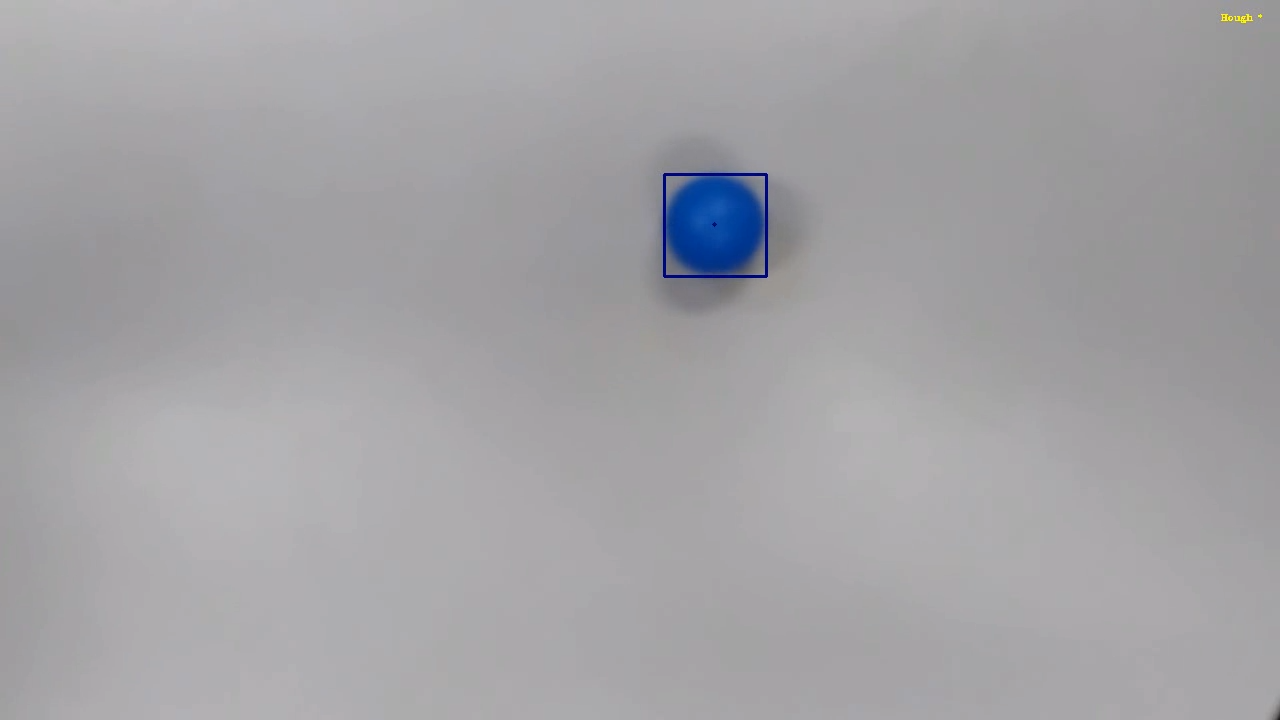
\includegraphics[scale=0.15]{images/single_color}}
    \caption{Detection of a colored ball.}\label{fig:single_color}
  \end{figure}

  The color detection applied to every frame was able to track the ball
  throughout the camera's view. This solution showed itself insufficient when
  some objects were introduced, with different shapes other than of a sphere but
  same color as the ball.

  \bigbreak{}
  \textbf{Two different color tracking:}
  \bigbreak{}

  The goal was to track each colored ball throughout the camera's view, not ever
  mistaking one with another.

  \begin{figure}[!h]
    \centering
    \setlength{\fboxsep}{1pt}
    \setlength{\fboxrule}{1pt}
    \fbox{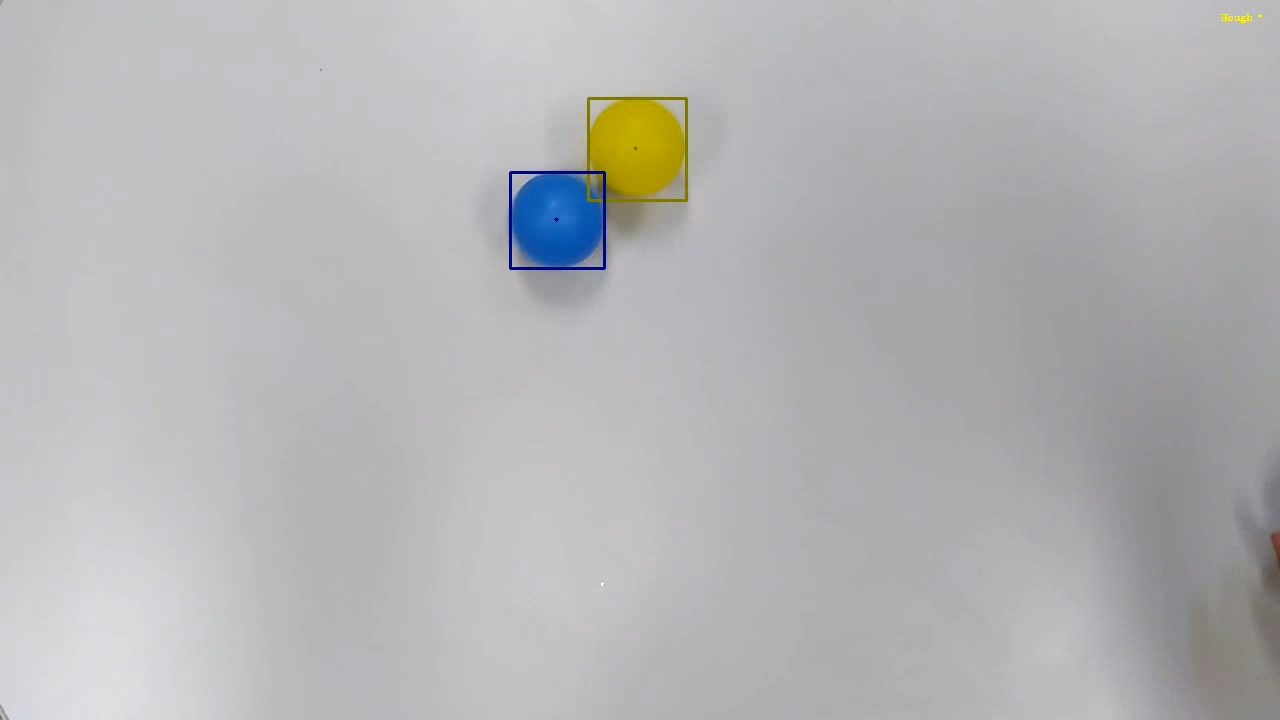
\includegraphics[scale=0.15]{images/diff_color}}
    \caption{Detection of two balls with different colors.}\label{fig:diff_color}
  \end{figure}

  The fine tuning of the colors enabled the solution to isolate one ball from
  the other, tracking them throughout the camera's view. This limits the
  solution to be tuned at every application, indoor  and outdoor needs
  distinct calibrations.

  \bigbreak{}
  \textbf{Two same color tracking:}
  \bigbreak{}

  The goal was to track each ball throughout the camera's view, not ever
  mistaking one with another, now differentiating between two balls of the same
  color.

  \begin{figure}[!h]
    \centering
    \setlength{\fboxsep}{1pt}
    \setlength{\fboxrule}{1pt}
    \fbox{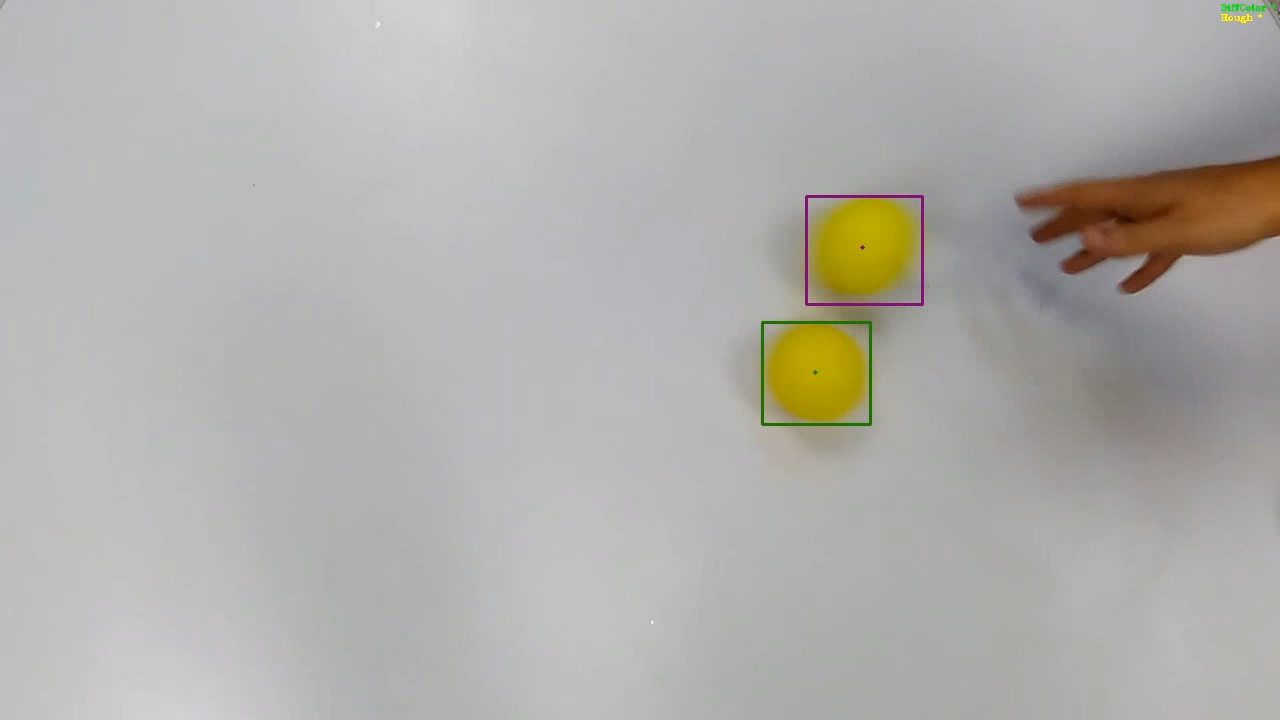
\includegraphics[scale=0.15]{images/same_color}}
    \caption{Detection of two balls with the same color.}\label{fig:same_color}
  \end{figure}

  The size of the connected components regions found in the mask were used the
  discriminate between the balls, the ratio between the first and second was
  used and enabled the tracking to work, the solution is limited when the object
  of interest moves away from the camera and becomes too small to pass the
  threshold.

  \bigbreak{}
  \textbf{Ball tracking alongside with other shapes:}
  \bigbreak{}

  The goal was to track a ball in a setup with many objects with different
  shapes, but same color as the ball.

  \begin{figure}[!h]
    \centering
    \setlength{\fboxsep}{1pt}
    \setlength{\fboxrule}{1pt}
    \fbox{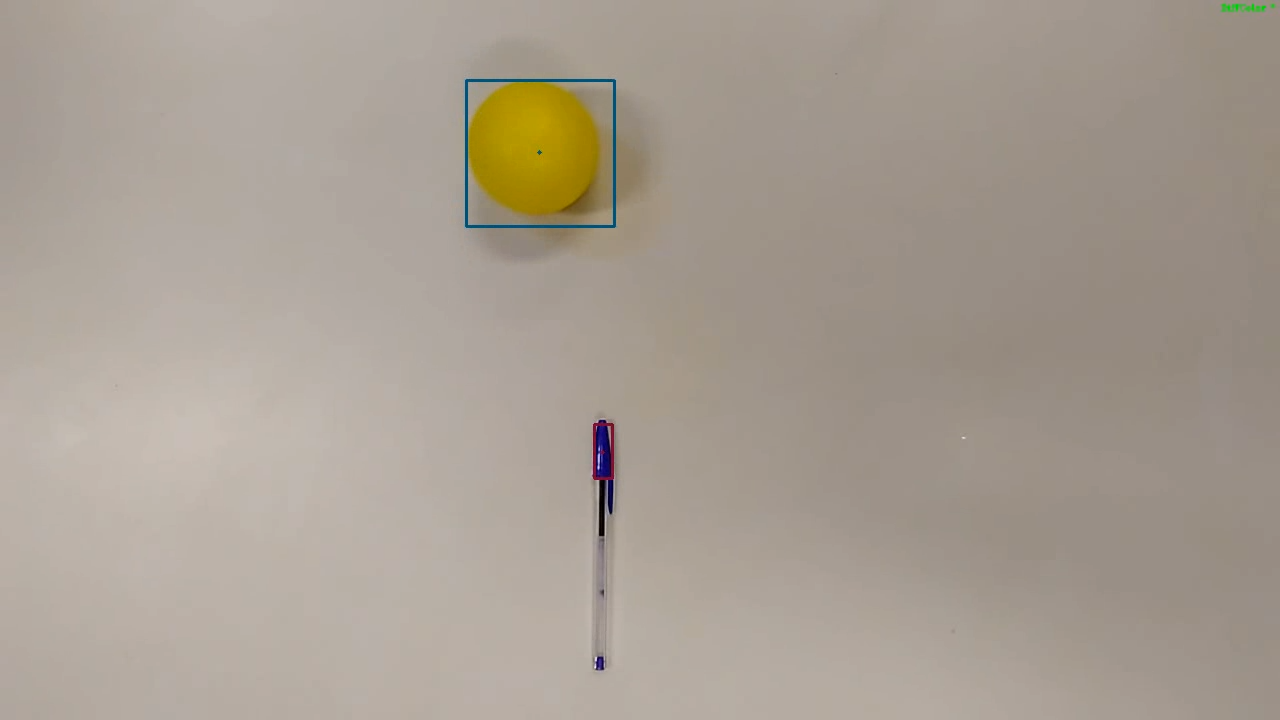
\includegraphics[scale=0.15]{images/not_hough}}
    \caption{Detection before the Hough Circle Transform.}\label{fig:not_hough}
  \end{figure}

  As seen in Figure~\ref{fig:not_hough} the solution wasn't able to
  differentiate the ball from the pen top.

  \begin{figure}[!h]
    \centering
    \setlength{\fboxsep}{1pt}
    \setlength{\fboxrule}{1pt}
    \fbox{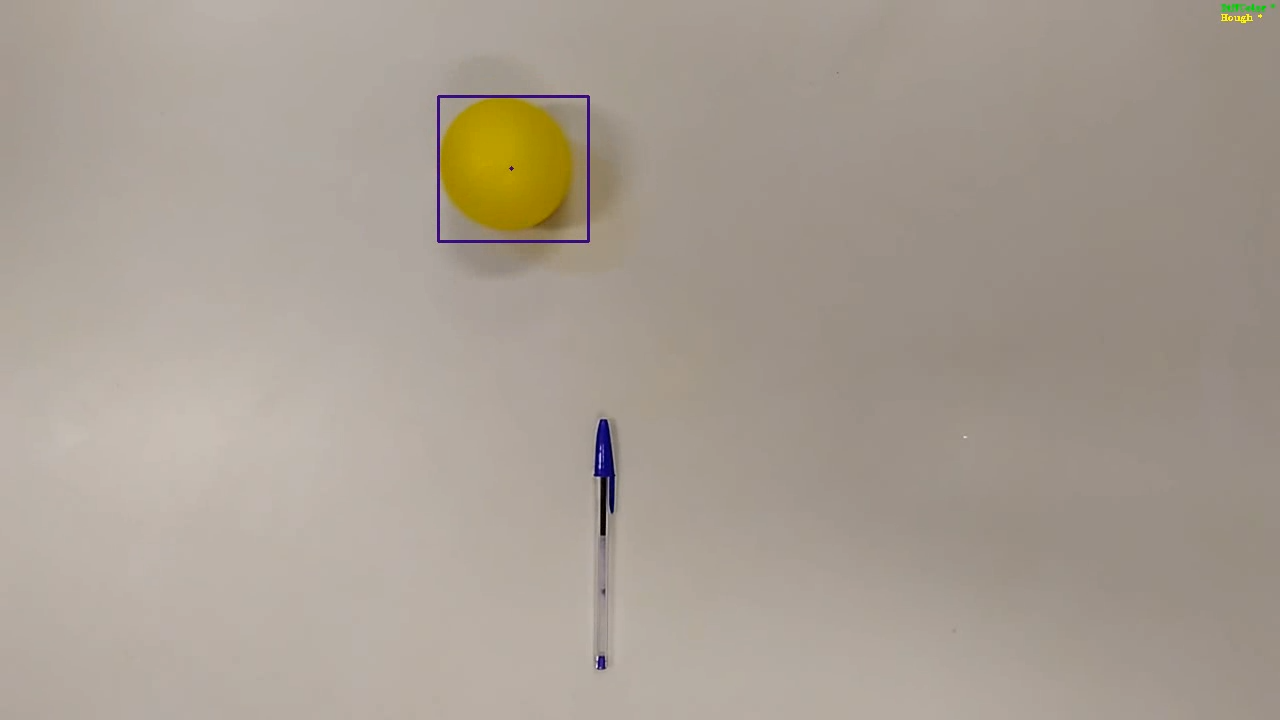
\includegraphics[scale=0.15]{images/yes_hough}}
    \caption{Detection after the Hough Circle Transform.}\label{fig:yes_hough}
  \end{figure}

  In Figure~\ref{fig:yes_hough} using the Hough Circle Transform the solution
  was able to ignore the pen top and track only the ball shaped object. This
  solution is still limited by the time it took to adjust the parameters into
  differentiate a pen top and a ball.

  \bigbreak{}
  \textbf{Motion flow tracking compared with color tracking:}
  \bigbreak{}

  The goal was to compare both solutions, Lucas Kanade motion flow tracking and
  every frame color detection.

  \begin{figure}[!h]
    \centering
    \setlength{\fboxsep}{1pt}
    \setlength{\fboxrule}{1pt}
    \fbox{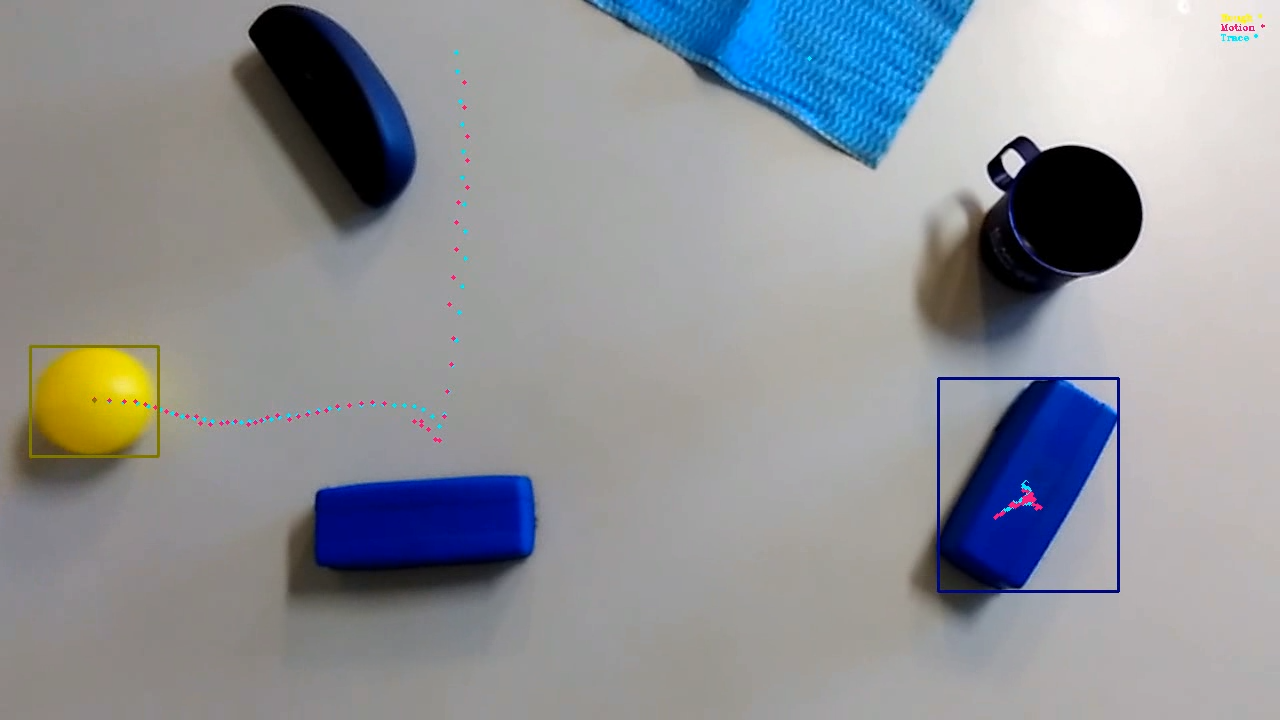
\includegraphics[scale=0.15]{images/motion_5}}
    \caption{Lucas Kanade motion flow applied every 30 frames.}\label{fig:motion_30}
  \end{figure}

  Using the Lucas Kanade motion flow the solution would only apply the color
  detection every $N$ frames, this gap between detection speed up the tracking
  and enabled it to perform in real time (greater than 20 fps). The precision of
  the tracking depended on the gap size, and this experiment showed that a gap
  of 30 frames was too large.

  \begin{figure}[!h]
    \centering
    \setlength{\fboxsep}{1pt}
    \setlength{\fboxrule}{1pt}
    \fbox{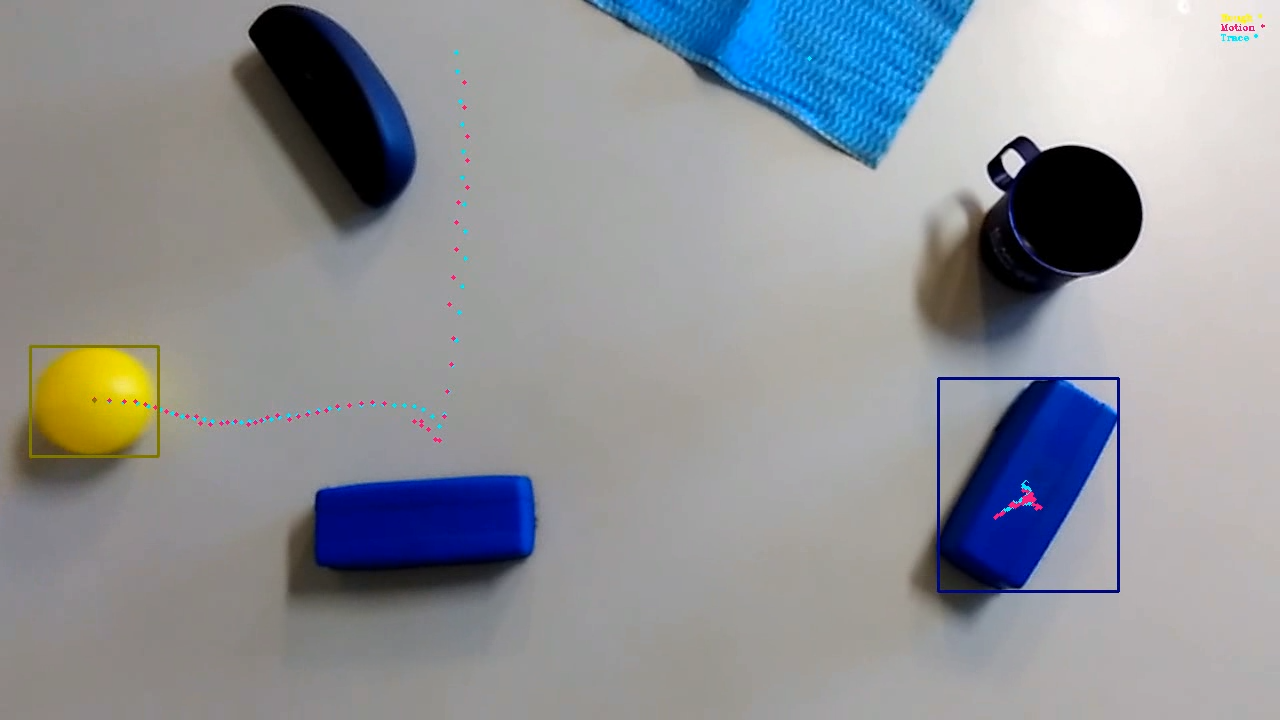
\includegraphics[scale=0.15]{images/motion_5}}
    \caption{Lucas Kanade motion flow applied every 5 frames.}\label{fig:motion_5}
  \end{figure}

  Using a 5 frames gap the precision of the tracking was close to the color
  tracking and the solution was still fast enough to operate in real time.
  Although this solution couldn't keep tracking of the ball when it was occluded.

  \bigbreak{}
  \textbf{Occlusion tracking:}
  \bigbreak{}

  The goal was to compare the LK motion flow tracking and kalman filter
  tracking, both applied towards a occlusion scenario.

  \begin{figure}[!h]
    \centering
    \setlength{\fboxsep}{1pt}
    \setlength{\fboxrule}{1pt}
    \fbox{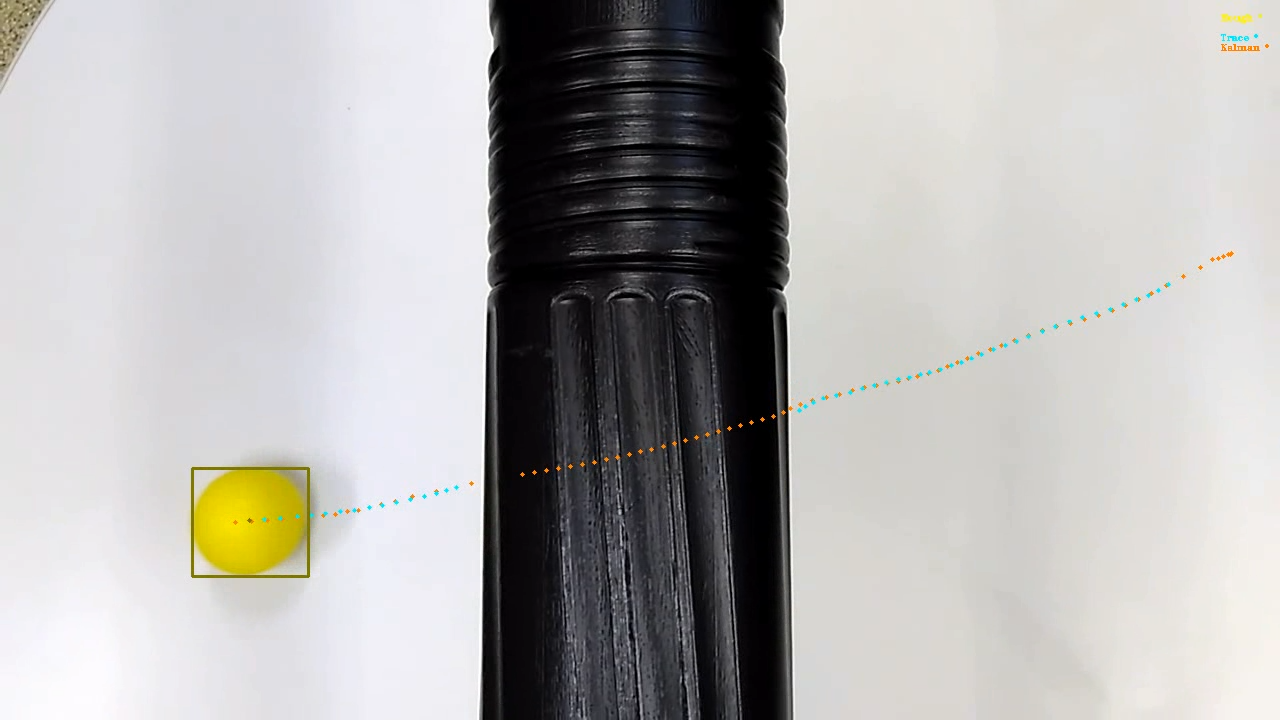
\includegraphics[scale=0.15]{images/occlusion}}
    \caption{Kalman filter applied to overcome occlusion.}\label{fig:occlusion}
  \end{figure}

  The solution was able to overcome occlusion when the kalman filter was used in
  such scenarios, since it was able to estimate the ball's trajectory. The
  filter worked best with low speeds and couldn't estimate a position if the
  ball changed directions whilst occluded.

  \bigbreak{}
  \textbf{Real world tracking:}
  \bigbreak{}

  The goal was to hard test all the features implemented in a real world
  scenario to evaluate their precision.

  \begin{figure}[!h]
    \centering
    \setlength{\fboxsep}{1pt}
    \setlength{\fboxrule}{1pt}
    \fbox{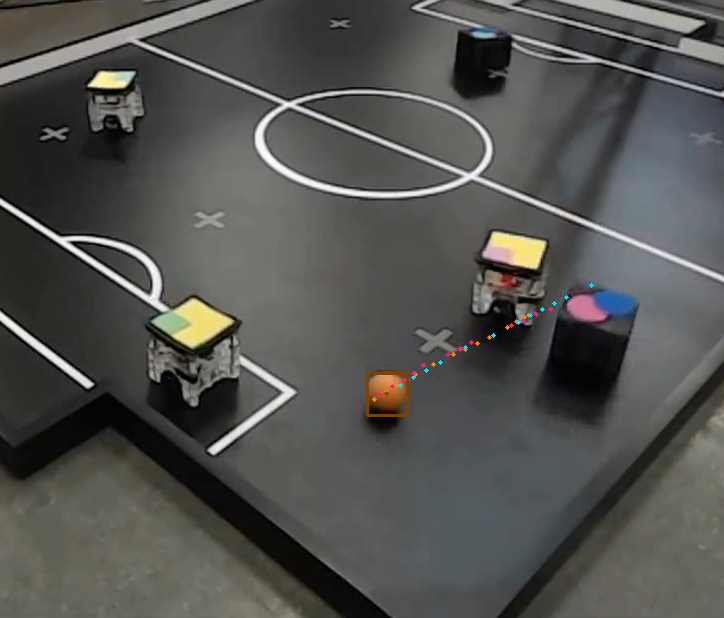
\includegraphics[scale=0.15]{images/robocup_1}}
    \caption{All features applied in a Robocup soccer match.}\label{fig:robocup_1}
  \end{figure}

  When applied to a real world scenario the solution can keep tracking up to a
  point, it fails whenever the ball changes direction while occluded, or when
  the ball moves too fast.

%-------------------------------------------------------------------------
  \section{Conclusion}\label{sec:conclusion}

  Even though the classic methods were able to track and overcome some of the
  challenges presented in this report they couldn't keep their precision in a real world
  scenario. Some other approaches to detect and track are needed for scenarios
  like a volleyball match, where the ball is white and the people watching the
  game are often caught in the camera along side with the game. Other works used deep
  learning to train a network into detecting the ball, some used a physics model
  to calculate the parabolic trajectory of the ball and some used completely
  different clues, like the fact that a basketball player moves differently from
  the others when he/she has the ball in hands.

  To go through the classic methods many of the course's topics were covered and
  applied, clearing our sights towards their weakness, strength and how they are
  applied. It is instigating to think the power that a neural network would have
  in such context, and realize from other works the vast number of ways to
  tackle a single problem.

{\small
\bibliographystyle{ieee}
\bibliography{egbib}
}

\end{document}
